
\documentclass{bmcart}


\usepackage[utf8]{inputenc} %unicode support
%\usepackage{caption}
\usepackage{graphicx}
\usepackage{bm}
\usepackage{subfigure}
\usepackage{multirow}
\usepackage{algorithm}
\usepackage{algorithmic}
\usepackage{array}
\usepackage{subfigure}
\usepackage{mathrsfs}
\usepackage{epstopdf}
\usepackage{amsmath}
\usepackage{enumerate}
\usepackage{amsmath}
%\usepackage{underscore}
\usepackage{booktabs,caption,fixltx2e}
\usepackage[flushleft]{threeparttable}
\startlocaldefs
\endlocaldefs


%%% Begin ...
\begin{document}
%%% Start of article front matter
\begin{frontmatter}

\begin{fmbox}
\dochead{Research}

\title{Consistent Multiple Nonnegative Matrix Factorization with Hierarchical Information for Gene Functional Modules Mining}


\author[
   addressref={aff1,aff2},                   % id's of addresses, e.g. {aff1,aff2}
   %corref={aff1},                       % id of corresponding address, if any
   %noteref={n1},                        % id's of article notes, if any
   email={ygzhang@mail.nankai.edu.cn}   % email address
]{\inits{YGZ}\fnm{YaoGong} \snm{Zhang}}
\author[
   addressref={aff1,aff2},
   email={xuyingjie@mail.nankai.edu.cn}
]{\inits{YJX}\fnm{YingJie} \snm{Xu}}
\author[
   addressref={aff1,aff2},
   email={nkufanxin@mail.nankai.edu.cn}
]{\inits{XF}\fnm{Xin} \snm{Fan}}
\author[
   addressref={aff1,aff2},
   email={hongyuxiang@mail.nankai.edu.cn}
]{\inits{YXH}\fnm{YuXiang} \snm{Hong}}
\author[
   addressref={aff1,aff2},
   email={hezhicheng@mail.nankai.edu.cn}
]{\inits{ZCH}\fnm{ZhiCheng} \snm{He}}
\author[
   addressref={aff1,aff2},
   email={huangyl@nankai.edu.cn}
]{\inits{YLH}\fnm{YaLou} \snm{Huang}}
\author[
   addressref={aff1,aff2},
   corref={aff1},                       % id of corresponding address, if any
   email={xiemq@nankai.edu.cn}
]{\inits{MQX}\fnm{MaoQiang} \snm{Xie}}

\address[id=aff1]{%
  \orgname{College of Software, NanKai University},
  %\street{D\"{u}sternbrooker Weg 20},
  \postcode{300350}
  \city{TianJin},
  \cny{China}
}
\address[id=aff2]{%                           % unique id
  \orgname{College of Computer and Control Engineering, NanKai University}, % university, etc
  %\street{WeiJin Road},                     %
  \postcode{300350}                                % post or zip code
  \city{TianJin},                              % city
  \cny{China}                                    % country
}


%\begin{artnotes}
%%\note{Sample of title note}     % note to the article
%\note[id=n1]{Equal contributor} % note, connected to author
%\end{artnotes}

\end{fmbox}% comment this for two column layout

\begin{abstractbox}

\begin{abstract} % abstract
\parttitle{Background} %if any
An increasing amount of genome-phenome association data, has provided us an unprecedented chance to globally explore the underlying genetic mechanisms and understand the regularization between genes and diseases with a deeper sight perspective. Gene modules, which reveals the interactions between genes and help researchers to identify candidate genes as drug targets et,al., has always been a significant and valuable problem by utilizing genome-phenome association data. Nevertheless, the hierarchical structure of phenotype ontology has been rarely leveraged by previous gene clustering studies, the properties of genes, diseases and their relationships has not been fully explored, which may result in missing the chance to discover the crucial fact in biology. Thereby, it is challenging to utilize this neglected hierarchical character of phenotype ontology to gain understanding of biological system.\\
\textbf{Results:}
We propose a novel method, Consistent Multiple Nonnegative Matrix Factorization (CMNMF), to utilize the hierarchical structure of phenotype ontology to cluster genes in genome-phenome association data on mouse. The CMNMF method, constrains the gene cluster matrix to remain consistent while it interacts with different phenotype ontology levels in decomposing the genome-phenome association matrix, meanwhile it restricts the similarity of phenotype pairs to satisfy the hierarchical structure.  \\
\textbf{Conclusions:}
The performance of our proposed method and other baselines (including HAC, Kmeans, Kernel-Kmeans, LDA, NMF,ColNMF) are evaluated on $F_1$ , $Jaccard\ Index$, $Rand\ Index$ and $GO_{rate}$. The results show the effectiveness of our proposed method compared with other baselines. Additionally, we conduct the Supervised Consistent Multiple Nonnegative Matrix Factorization(S-CMNMF) to do multi-label gene classification problem, S-CMNMF beats other baselines as well.
Our work explores the crucial impact of hierarchical structure of phenotype ontology in gene clustering, and we show our proposed method outperforms baselines in both unsupervised and supervised manner, which provides a new perspective to conduct research on biological data exploration.\\
\textbf{Availability:} \texttt{https://github.com/nkiip/CMNMF}\\
%\textbf{Contact:} {name@bio.com}{name@bio.com}\\
%\parttitle{Second part title} %if any
%Text for this section.
\end{abstract}

\begin{keyword}
\kwd{NMF}
\kwd{Gene modules mining}
\kwd{Hierarchical information}
\end{keyword}


\end{abstractbox}
%
%\end{fmbox}% uncomment this for twcolumn layout

\end{frontmatter}


\section*{Background}
With the development of technology, biomedical researchers has collected a large amount of valuable biological data by these years, especially the genome-phenome association data on mouse, whose research achievement may transfer to human disease study, it is of great significance for drug development and disease treatment. Thereby it is necessary and essential for researchers to have a deeper sight investigation on mouse data. The international database resources such as Mouse Genome Informatics (MGI)\footnote{http://www.informatics.jax.org/}, Kyoto Encyclopedia of Genes and Genomes (KEGG)\footnote{http://www.genome.jp/kegg/} etc. provide more and more multiple types of mouse biological data. However, how to integrate and utilize those data in a effective way to discover the underlying patterns and biological mechanism is still a challenging issue, which has drawn growing attention in the literature.

It is well known that genes in mammal genomes are usually organized into groups functionally associate with phenotype groups\cite{XuanH2015,Yao2011,Lage2007,Oti2006}. Identification of modules of functionally related genes is a crucial first step towards dissecting the regulatory circuitry underlying biological processes. Co-regulated or functionally related genes are likely to reveal themselves by associations with different diseases. These modules may provide clues about the main biological processes associated to different physiological states and provide guidance for candidate genes of genetic diseases.

Phenotypes, is the composite of an organism's observable characteristics or traits, results from the expression of an organism's genes as well as the influence of environmental factors and the interactions between the two\cite{McKusick2007,PhilipGroth2006}. The key to achieving desired gene modules such as favorable disease treatment outcomes lies in the understanding of the relation between phenotypes and the biological roles of genes \cite{Sawyers2008,Rubin2008,Edwards2004}. Phenotype ontology was created to serve as a standardized vocabulary of phenotypic abnormalities that have been seen in diseases, can be used as a computational representation of phenotype knowledge based upon a hierarchical structure\cite{Robinson2014,Kohler2014,Smith2009}. This kind of structure provides researchers extra information about the relationships between phenotype pairs. Whereas, as far as we know, the hierarchical structure of phenotype ontology has not been utilized for gene module identification, the phenotype ontology in different levels reflects underlying associations while interacting with disease genes. With taking advantage of this character, it gives us a new perspective to explore the patterns behind the biological data.

Much research studies have been conducted on integration of multiple sources of biological data to mine the hidden patterns and the relationships between distinct data sources. Some procedures based on gene expression profiles, seeking to map different experimental data types, such as gene expression, miRNA expression, and copy number variation to a common space of known biological pathways or sets\cite{Khatri2012,Mitrea2013}. Zhang\cite{Zhang2011} focuses on integrating multiple type genomic data to identify microRNA-gene regulatory modules for cancers. Extended Dirichlet mixture model\cite{Lock2013} and principal component analysis\cite{Lock2013a} make the distinction between common and distinct effects across sources. Some studies incorporated clinical phenotype data to increase the ability of identifying new disease-associated genes\cite{Hwang2012,Lage2007,Li2010,Vanunu2010,Wu2008a,Wu2008b}
%(Hwang et al., 2012; Lage et al., 2007; Li and Patra, 2010; Vanunu et al., 2010; Wu et al., 2008, 2009)("Phenome-driven disease genetics prediction toward drug discovery")
, a key assumption in these methods is that similar disease phenotypes reflect overlapping genetic causes\cite{Houle2010}.
%(Houle et at.,2010)
%("Phenome-driven disease genetics prediction toward drug discovery").
 Because some data contains specific structures behind it, thus some structure based methods are proposed and all achieve good results. In the collaborative recommendation task, some grouping strategies based on structure information are proposed, such as grouping users by social networks, grouping items by defined hierarchy or grouping both of them \cite{Wang2014,Ma2008,AliMashhoori2012}. HPMF\cite{Shan2012} focuses on predicting missing traits for plants which incorporates hierarchical phylogenetic information into matrix factorization. The results of these methods demonstrate that considering auxiliary structured information can bring a better performance.

In this study, we developed a novel NMF based approach Consistent Multiple Nonnegative Matrix Factorization (CMNMF) to combine structured phenotype ontology data on mouse disease phenotype to predict disease-associated gene modules. The key ideas of our method are that the same gene should be active in the same modules when interacting with phenotypes from different levels of the hierarchical phenotype ontology, and the similarity of phenotype pairs, which has parent-child relationships, should keep high in the hierarchical structure. To demonstrate the approach, we conduct our proposed method on a sampled data first, and series of measurements with other baselines on gene clustering task in an unsupervised way, the performance of our CMNMF on $F_1$ $measure$, $Rand$ $Index$, $Jaccard\ Index$, and $GO_{rate}$ outperform other baselines, including Kmeans, Kernel-Kmeans\cite{Dhillon2004}, HAC\cite{Ward1963}, ColNMF\cite{Singh2008}, NMF\cite{Lee1999}, LDA\cite{Blei2003}. Besides, we extend CMNMF with gene classification prior, which we call Supervised CMNMF(S-CMNMF) on gene classification task, the $AUC$ score demonstrates the advantages of S-CMNMF over ColNMF, and LP\cite{Raghavan2007}.
\begin{figure}[!t]
  \centering
  \begin{minipage}{.80\linewidth}
  \centering
    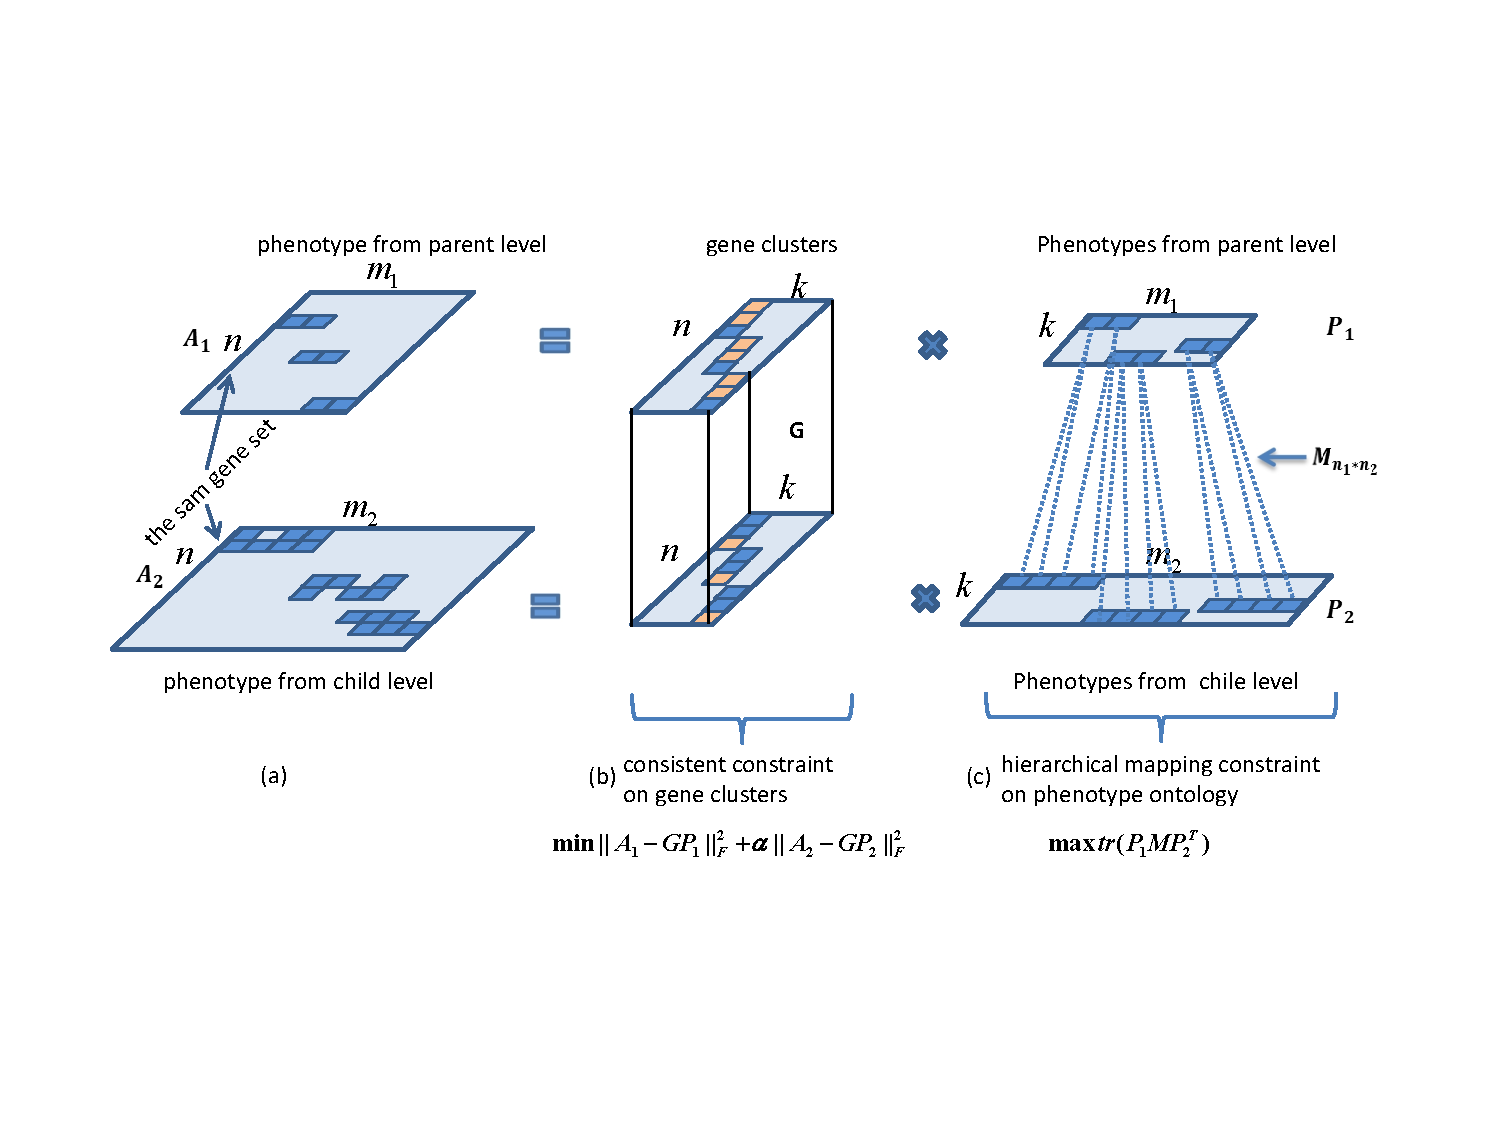
\includegraphics[width=\linewidth]{DrawPictures/module2.pdf}
  \end{minipage}
  \caption{Overview of the proposed CMNMF model}
  \label{fig:model}
\end{figure}
%The remainder of the paper is organized as follows. We present our consistent multiple nonnegative matrix factorization framework in Section 2. Section 3 reports some experiments and discussions. Followed with conclusion and future work in section 4.

\section*{Method}
Figure \ref{fig:model} illustrates the framework of the Consistent Multiple Non-negative Matrix
Factorization with hierarchical constraints of phenotype ontology to identify gene modules.
We designed an objective function with three components. The first and second components are based on non-negative genome-phenome association data with respect to distinct level phenotype ontologies. The third one considers the effects of interactions from phenotype ontology. By optimizing this objective function, we obtain a consistent decomposition of two genome-phenome association matrix, which reveals gene functional modules inherent in genome-phenome association data jointly.
\begin{table}[t!]
 \caption{Summary of notations.}\label{Tab:Notations}
%\processtable{Summary of notations.\label{Tab:01}} {
\begin{tabular}{|l|l|}
    \hline
    Notations & Explanations\\
    \hline\hline
    $\bm{A}$ & Genome-phenome association matrix with phenotype \\
    & from parent and child level\\
    $\bm{A}_1$ & Genome-phenome association matrix with phenotype\\
    & ontology from parent level\\
    $\bm{A}_2$ & Genome-phenome association matrix with phenotype\\
    & ontology from child level\\
    $\bm{G}$ & Gene cluster membership\\
    $\bm{G}_0$ & Annotated gene cluster membership\\
    $\bm{P}_1$ & Phenotype cluster membership of parent level\\
    $\bm{P}_2$ & Phenotype cluster membership of child level\\
    $\bm{M}$ & Phenotype ontologies relationship\\
    $n$ & Number of disease genes\\
    $m$ & Number of phenotype ontology in parent and child level\\
    $k$ & Number of latent clusters(e.g. classes)\\
    $m_1$ & Number of phenotype ontology in parent level\\
    $m_2$ & Number of phenotype ontology in child level\\
    \hline
  \end{tabular}
\end{table}

\subsection*{\textbf{Problem formulation}}
The notations and definitions used in the article are specified in Table \ref{Tab:Notations}.
We denote $\bm{A}_{(n \times m)}$ a binary gene-phenotype association matrix by $n$ genes and $m$ phenotypes, where $\bm{A}_{ij}$ is set with 1 for known association and 0 otherwise. The goal of factorizing matrix $\bm{A}$ based on NMF\cite{DanielD.Lee2001} is to derive gene functional clusters . The loss of it can be defined as:
\begin{equation}\label{equ:NMF}
\mathop{min}_{{\bm{P},\bm{G}}} \|\bm{A}-\bm{GP}\|^{2}_{F}
\end{equation}
Where $\bm{G}_{n\times k}$ and $\bm{P}_{k\times m}$ denotes gene clusters and phenotype clusters , respectively. The notation $||\bullet||_F$ means the $Frobenius$ norm of a matrix.

Based on multiplicative update rules\cite{DanielD.Lee2001}, we can get a non-negative solution of $\bm{G}$ and $\bm{P}$. The elements of $\bm{G}$ can be interpreted as latent modules associated with genes, thus a couple of clusters of genes are achieved with a good interpretation on NMF.

However, the NMF method in this form has not taken the hierarchical mapping information of phenotype ontology into consideration. To address this problem, we design a loss function with two aspects for formulating the loss with hierarchical information of phenotype ontologies:
\begin{itemize}
\item The first aspect is a consistent constraint on gene cluster, the reason is intuitive, one gene interacts with a child phenotype ontology, it should interact with the child ontology's parent phenotype ontology, because parent phenotype ontologies are generalization of child phenotype ontologies, the child phenotype ontologies are specification of parent phenotype ontologies (\emph{e.g.} MP2110: abnormal digit morphology, coming from level 4; MP564: syndactyly, coming from level 5). Figure \ref{fig:model}(a) shows the gene clustering results on general and specific phenotype ontology level, on which we put a consistent constraint.
\item The second component is a hierarchical mapping constraint between phenotype ontologies from parent level and ones from child level. Fig. \ref{fig:model}(b). Because phenotype ontologies coming from the adjacent level, there should exist strong relationships between these parent-child ontologies pairs, in which we apply hierarchical mapping constrains to demonstrate the relationships between them. The clusters of phenotype ontologies from different levels should be consistent as well.
\end{itemize}
By optimizing these two components, our CMNMF (Consistent Multiple Non-negative Matrix Factorization) algorithm is proposed to obtain consistent gene clusters.

\subsection*{\textbf{Loss Functions for Penalizing Inconsistence}}
Motivated by above consistent assumption, we extract phenotype ontologies from two adjacent levels, and two gene-phenotype association matrices $(\bm{A}_1)_{n\times m_1}$ and $(\bm{A}_{2})_{n\times m_2}$ are extracted from gene-phenotype text file. We assume that the factorizations on  $\bm{A}_{1}$ and $\bm{A}_{2}$ for the gene cluster should be consistent, although the genes are annotated by adjacent level phenotype ontologies. In our work, we use a common basis gene cluster matrix $\bm{G}_{n\times k}$ to achieve this goal. The representation of the data can be derived by optimizing the following quadratic objective function:
\begin{equation}
{L_C} = \mathop {\min }\limits_{\bm{G},{\bm{P}_1},{\bm{P}_2}} \left\| \bm{A}_1 - \bm{G{P}}_1 \right\|_F^2 + \alpha \left\| {\bm{A}_2} - \bm{GP}_2 \right\|_F^2,
\end{equation}
where $\alpha$ is a parameter to balance the factorization error from different levels.

For the hierarchical mapping constraints on phenotype ontologies, loss function in Equation (\ref{equ:L_H}) is used to encourage the interactions between phenotypes from parent level and child level.
\begin{equation}\label{equ:L_H}
{L_H} = \sum\limits_{ij} {{\bm{M}_{ij}}} {(\bm{P}_1^{(i)})^T}\bm{P}_2^{(j)} = tr({\bm{P}_1}\bm{MP}_2^T),\
\end{equation}
where $\bm{M}_{m_1\times m_2}$ denotes the hierarchical mapping relation matrix between phenotype ontologies from different levels. $\bm{M}_{ij}=1$, if phenotype $i$ and phenotype $j$ have a parent-child relationship, otherwise 0. We enforce hierarchical mapping constraints by maximizing the mapping between the phenotype ontologies in gene-phenotype network $\bm{A}_{1}$ and $\bm{A}_{2}$.

\subsection*{\textbf{Regularization by Sparse Constraint}}
Since the known gene-phenotype associations are sparse and only cover a part of genes and phenotypes, the regularization with $L_2$ norm is proposed to control the sparseness of $\bm{G}$, $\bm{P}_1$ and $\bm{P}_2$. The coefficients ${\lambda_1}$ and $\lambda_2$ balance the regularization terms. Finally, the framework of regularized CMNMF with sparse constraint is to minimize the loss function formulated as follows:
\begin{equation}\label{equ:R-CMNMF}
\begin{split}
%\mathop {\min }\limits_{G,{P_1},{P_2}}
L=
&\left\| {{\bm{A}_1} - \bm{G}{\bm{P}_1}} \right\|_F^2 + \alpha \left\| {{\bm{A}_2} - \bm{G}{\bm{P}_2}} \right\|_F^2 - \gamma tr({\bm{P}_1}\bm{MP}_2^T)\\
&{\rm{ + }}{\lambda _1}\left\| \bm{G} \right\|_F^2{\rm{ + }}{\lambda _2}(\left\| {{\bm{P}_1}} \right\|_F^2{\rm{ + }}\left\| {{\bm{P}_2}} \right\|_F^2)\\
&\mathrm{s.t. }\quad \sum_j\bm{G}_{ij}=1,\quad \sum_i{(\bm{P}_1)}_{ij}=1,\quad \sum_i{(\bm{P}_2)}_{ij}=1
\end{split}
\end{equation}
%&\mathrm{s.t. }\qquad {\rm{G}} \ge {\rm{0, }}\quad{{\rm{P}}_1}{\rm{, }} {{\rm{P}}_2} \ge 0
where $\alpha ,\gamma ,{\lambda _1},{\lambda _2}$ are parameters to balance the trade of each component.

\subsection*{\textbf{Optimization Framework for CMNMF}}
We extend the optimization algorithms of \cite{Singh2008}. The strategy to solve the problem is to optimize the objective loss function with respect to one variable while keep the other variables fixed.

\subsubsection*{\textbf{Computation of $G$ in CMNMF}}
We fix variables $\bm{P}_1$ and $\bm{P}_2$,
 %solving Eq(\ref{equ:S-CMNMF}) with respect to $G$ is equivalent to minimizing the following function:
%\begin{equation}\label{obj:obj_G}\nonumber
%\begin{split}
%&L(G)=\left\| {{A_1} - GP_1} \right\|_F^2 + \alpha \left\| {{A_2} - G{P_2}} \right\|_F^2
%     +{\lambda _1}\left\| G \right\|_F^2\\
%     &\mathrm{s.t. }\quad \sum_jG_{ij}=1,G\ge 0
%\end{split}
%\end{equation}
using the Karush-Kuhn-Tucher (KKT) conditions $\bm{\Phi}_{ij}\bm{G}_{ij}=0$, the partial derivative of Equation (\ref{equ:R-CMNMF}) with respect to $\bm{G}$ is:
\begin{equation}\label{equ:G_gradient}\nonumber
\begin{split}
\frac{\partial{L}}{\partial{\bm{G}}}=
&-2(\bm{A}_1{\bm{P}_1^T} - \bm{G}{\bm{P}_1}{\bm{P}_1^T})-2\alpha(\bm{A}_2{\bm{P}_2^T} - \bm{G}{\bm{P}_2}{\bm{P}_2^T})+2\lambda_1\bm{G}+\bm{\Phi}
\end{split}
\end{equation}
The multiplicative update rule is:
\begin{equation}\label{equ:updating_G}\nonumber
\bm{G}_{ij}\leftarrow \bm{G}_{ij}
\frac{(\bm{A}_1\bm{P}_1^T+\alpha \bm{A}_2\bm{P}_2^T)_{ij}}
{(\bm{GP}_1\bm{P}_1^T+\alpha \bm{GP}_2\bm{P}_2^T+\lambda_1\bm{G})_{ij}}
\end{equation}
To satisfy the equality constraint, we normalize $\bm{G}_{ij}$ in rows.
%\begin{equation}\label{equ:updating_G}\nonumber
%G_{ij}\leftarrow \frac{G_{ij}}{\sum_{j}G_{ij}}
%\end{equation}

%%%%%%%%%%%%%%% Computation of $P_1$ and $P_2$ %%%%%%%%%%%%%%%%%%%%%%%%
\subsubsection*{\textbf{Computation of $\bm{P}_1$ and $\bm{P}_2$ in CMNMF}}
When $\bm{G}$ is computed,
%solving Eq(\ref{equ:S-CMNMF}) with respect to $P_1$  and $P_2$ is equivalent to minimizing the following function:
%\begin{equation}\label{equ:obj_P1}\nonumber
%\begin{split}
%&L(P_{1})=\left\| {{A_1} - GP_1} \right\|_F^2 - \gamma tr({P_1}MP_2^T)+{\lambda _2}(\left\| {{P_1}} \right\|_F^2 )\\
%   &\mathrm{s.t. }\quad \sum_i (P_1)_{ij}=1,P_1\ge 0\\
%&L(P_{2})=\alpha\left\|A_2 - GP_2\right\|_F^2 - \gamma tr(P_1MP_2^T)+{\lambda _2}(\left\|P_2\right\|_F^2 )\\
%   &\mathrm{s.t. }\quad \sum_i (P_2)_{ij}=1,P_1\ge 0
%\end{split}
%\end{equation}
the partial derivative of Equation (\ref{equ:R-CMNMF}) with respect to $\bm{P}_1$ and $\bm{P}_2$ are:
\begin{equation}\label{equ:P1_gradient}\nonumber
\begin{split}
&\frac{\partial{L(\bm{P}_1)}}{\partial{\bm{P}_1}}=
-2(\bm{G}^T\bm{A}_1-{\bm{G}^T\bm{GP}_1})-\gamma \bm{P}_2\bm{M}^T +2\lambda_2\bm{P}_1+\bm{\Omega}\\
&\frac{\partial{L(\bm{P}_2)}}{\partial{\bm{P}_2}}=
-2\alpha(\bm{G}^T\bm{A}_2-{\bm{G}^T\bm{GP}_2})-\gamma \bm{P}_1\bm{M} +2\lambda_2\bm{P}_2+\bm{\Psi}
\end{split}
\end{equation}
Using the KKT conditions
 $\bm{\Omega}_{ij}(\bm{P}_1)_{ij}=0 , \bm{\Psi}_{ij}(\bm{P}_2)_{ij}=0$, the multiplicative update rule is(note that when we compute $\bm{P}_1$, we take $\bm{P}_2$ fixed, vise versa):
\begin{equation}\label{updating_P}\nonumber
\begin{split}
&(\bm{P}_1)_{ij}\leftarrow (\bm{P}_1)_{ij}
\frac{(\bm{G}^T\bm{A}_1+\frac{1}{2}\gamma \bm{P}_2\bm{M}^T)_{ij}}
{(\bm{G}^T\bm{GP}_1+\lambda_2\bm{P}_1)_{ij}}\\
&(\bm{P}_2)_{ij}\leftarrow (\bm{P}_2)_{ij}
\frac{(\alpha \bm{G}^T\bm{A}_2+\frac{1}{2}\gamma \bm{P}_1\bm{M})_{ij}}
{(\alpha \bm{G}^T\bm{GP}_2 + \lambda_2\bm{P}_2)_{ij}}
\end{split}
\end{equation}
To satisfy the equality constraint, we normalize $(\bm{P}_1)_{ij}$ and $(\bm{P}_2)_{ij}$ in columns.
%as
%\begin{equation}\label{equ:updating_P2}\nonumber
%\begin{split}
%(P_1)_{ij}\leftarrow \frac{(P_1)_{ij}}{\sum_{i}(P_1)_{ij}}, \quad
%(P_2)_{ij}\leftarrow \frac{(P_2)_{ij}}{\sum_{i}(P_2)_{ij}}
%\end{split}
%\end{equation}

%%%%%%%%%%%%%%%%%%%%%%%%%%% Computation of $P_2$ %%%%%%%%%%%%%%%%%%%%%%%%%
\subsection*{\textbf{Optimization framework of Supervised CMNMF}}
By considering prior gene classification prior, our proposed CMNMF can be utilized for another task ,multi-label gene classification problem as well. We call it Supervised CMNMF (S-CMNMF) as including gene classification prior. Thus, the loss function of S-CMNMF can be rewrite as:
\begin{equation}\label{obj:Sup-CMNMF}
\begin{split}
%\mathop {\min }\limits_{G,{P_1},{P_2}}
L_s =
&\left\| {{\bm{A}_1} - \bm{G}{\bm{P}_1}} \right\|_F^2 + \alpha \left\| {{\bm{A}_2} - \bm{G}{\bm{P}_2}} \right\|_F^2 +\beta\left\| {\bm{G} - {\bm{G}_0}}\right\|_F^2\\
&- \gamma tr({\bm{P}_1}\bm{MP}_2^T){\rm{ + }}{\lambda _1}\left\| \bm{G} \right\|_F^2{\rm{ + }}{\lambda _2}(\left\| {{\bm{P}_1}} \right\|_F^2{\rm{ + }}\left\| {{\bm{P}_2}} \right\|_F^2)\\
&\sum_j\bm{G}_{ij}=1,\quad \sum_i{(\bm{P}_1)}_{ij}=1,\quad \sum_i{(\bm{P}_2)}_{ij}=1
%\mathrm{s.t. }\qquad {\rm{  G}} \ge {\rm{0, }}\quad{{\rm{P}}_1}{\rm{, }} {{\rm{P}}_2} \ge 0,
\end{split}
\end{equation}

\subsubsection*{\textbf{Computation of $\bm{G}$ in Supervised CMNMF}}
We fix variables $\bm{P}_1$ and $\bm{P}_2$,
%solving Eq(\ref{obj:Sup-CMNMF}) with respect to $G$ is equivalent to minimize the following function:
%\begin{equation}\label{obj:sup_G}\nonumber
%\begin{split}
%&L_{s}(G)=\left\| {{A_1} - GP_1} \right\|_F^2 + \alpha \left\| {{A_2} - G{P_2}} \right\|_F^2
%     +\beta\left\| {G - {G_0}}\right\|_F^2+{\lambda _1}\left\| G \right\|_F^2\\
%     &\mathrm{s.t. }\quad \sum_jG_{ij}=1,G\ge 0
%\end{split}
%\end{equation}
the partial derivative of Equation (\ref{obj:Sup-CMNMF}) with respect to $\bm{G}$ is:
\begin{equation}\label{equ:G_gradient}\nonumber
\begin{split}
\frac{\partial{L_s}}{\partial{\bm{G}}}=
&-2(\bm{A}_1{\bm{P}_1^T} - \bm{G}{\bm{P}_1}{\bm{P}_1^T})-2\alpha(\bm{A}_2{\bm{P}_2^T} - \bm{G}{\bm{P}_2}{\bm{P}_2^T})+2\beta(\bm{G}-\bm{G}_0)+2\lambda_1\bm{G}+\bm{\Phi}
\end{split}
\end{equation}
Using the KKT conditions $\bm{\Phi}_{ij}\bm{G}_{ij}=0$, the multiplicative update rule is:
\begin{equation}\label{equ:updating_G}\nonumber
\bm{G}_{ij}\leftarrow \bm{G}_{ij}
\frac{(\bm{A}_1\bm{P}_1^T+\alpha \bm{A}_2\bm{P}_2^T+\beta \bm{G}_0)_{ij}}
{(\bm{GP}_1\bm{P}_1^T+\alpha \bm{GP}_2\bm{P}_2^T+\lambda_1\bm{G}+\beta \bm{G})_{ij}}
\end{equation}
To satisfy the equality constraint, we normalize $\bm{G}_{ij}$ in rows.
% as
%\begin{equation}\label{equ:updating_G}\nonumber
%G_{ij}\leftarrow \frac{G_{ij}}{\sum_{j}G_{ij}}
%\end{equation}

\subsubsection*{\textbf{Computation of $\bm{P}_1$ and $\bm{P}_2$ in Supervised CMNMF}}
Because the updating rules of supervised CMNMF for $\bm{P}_1$ and $\bm{P}_2$ are the same as CMNMF above, we would not present it here again.

\subsection*{\textbf{The Algorithm of CMNMF and Supervised CMNMF}}
The complete CMNMF algorithm is presented in \textbf{Algorithm \ref{alg:CMNMF}}. Our algorithm CMNMF can optimize the objective function iteratively by updating one variable while keep others fixed alternatively. As in the original NMF model, the cost of Equation (\ref{equ:NMF}) is not convex in $\bm{G}$ and $\bm{P}$ jointly, but it is convex in $\bm{G}$ for fixed $\bm{P}_1$ and $\bm{P}_2$, vice versa. the Lagrange multiplier method can be applicable here to give an iterative algorithm to guarantee the algorithm to converge to a local minima\cite{Zunyan2014}. For supervised CMNMF algorithm, we just need to change the update rule for $\bm{G}$ as we talked in \textup{Computation of $\bm{G}$ in Supervised CMNMF} part, the rest is the same as CMNMF.
\begin{algorithm}[t]
\caption{\textbf{CMNMF}}\label{alg:CMNMF}
\renewcommand{\algorithmicrequire}{\textbf{Input:}}
\renewcommand{\algorithmicensure}{\textbf{Output:}}
\label{alg:pf}
\begin{algorithmic}[1]
\REQUIRE gene-phenotype association matrix $\bm{A}_1$,$\bm{A}_2$, number of cluster dimensions $K$, and parameter $\alpha$,$\beta$,$\gamma$,$\lambda_1$,$\lambda_2$,
\ENSURE \text{model parameters} ${\bm{G}}, {\bm{P}_1},{\bm{P}_2}$
%\STATE $P \leftarrow \{(i,j)|q_i=q_j,y_i\succ y_j\}$
\STATE ${\bm{G}},{\bm{P}_1},{\bm{P}_2}$ $\leftarrow$ random values
%\STATE \text{stop$\_$condition:iterate number is more than $N$ or the change of objective function's value is less than $\varepsilon$}
%\STATE $ite = 1$
\REPEAT
    \STATE Update $\bm{G}_{ij}\leftarrow \bm{G}_{ij}\frac{(\bm{A}_1\bm{P}_1^T+\alpha \bm{A}_2\bm{P}_2^T)_{ij}}{(\bm{G}\bm{P}_1\bm{P}_1^T+\alpha \bm{G}\bm{P}_2\bm{P}_2^T+\lambda_1\bm{G})_{ij}}$
    \STATE Normalize $\bm{G}_{ij}\leftarrow \frac{\bm{G}_{ij}}{\sum_{j}\bm{G}_{ij}}$
    \STATE Update $(\bm{P}_1)_{ij}\leftarrow (\bm{P}_1)_{ij}\frac{(\bm{G}^T\bm{A}_1+\frac{1}{2}\gamma \bm{P}_2\bm{M}^T)_{ij}}{(\bm{G}^T\bm{G}\bm{P}_1+\lambda_2\bm{P}_1)_{ij}}$,
    $(\bm{P}_2)_{ij}\leftarrow (\bm{P}_2)_{ij}\frac{(\alpha \bm{G}^T\bm{A}_2+\frac{1}{2}\gamma \bm{P}_1\bm{M})_{ij}}
{(\alpha \bm{G}^T\bm{G}\bm{P}_2 + \lambda_2\bm{P}_2)_{ij}}$
    \STATE Normalize $(\bm{P}_1)_{ij}\leftarrow \frac{(\bm{P}_1)_{ij}}{\sum_{i}(\bm{P}_1)_{ij}}, \quad
(\bm{P}_2)_{ij}\leftarrow \frac{(\bm{P}_2)_{ij}}{\sum_{i}(\bm{P}_2)_{ij}}$

\UNTIL convergence
\RETURN ${\bm{G}},{\bm{P}_1},{\bm{P}_2}$
\end{algorithmic}
\end{algorithm}

\section*{Experiments Results and Analysis}
Our method's effectiveness on clustering gene modules is demonstrated on sampled gene-phenotype association matrixes at first by comparing the difference of conventional NMF and proposed CMNMF. We then execute CMNMF and four baseline methods on MGI mouse gene-phenotype ontology association data for mining mouse gene functional modules. Moreover, the evaluation of clustering results and parameter tuning are performed. Finally, gene ontology enrichment analysis is conducted to evaluate the biological significance of mined gene modules.

As an extension of CMNMF, by incorporating gene classification prior, our Supervised CMNMF show the good ability to classify multi-label problem compared with LP and ColNMF.
\subsection*{\textbf{Data Preparation}}
 The mouse gene-phenotype ontology associations are extracted from file ``MGI\_Geno\_Disease.rpt" (March-2015) downloaded from MGI \footnote{ftp://ftp.informatics.jax.org/pub/reports/MGI\_Geno\_Disease.rpt}, in which 5894 gene-phenotype associations at level 4 and 6817 associations at level 5 are kept. 2144 ontology terms at level 4 (parent level) and 2719 ontology terms at level 5 (child level)  are selected from the 10748 MP terms in the ``MPheno\_OBO.ontology''(November-2015) file\footnote{ftp://ftp.informatics.jax.org/pub/reports/MPheno\_OBO.ontology}. 2866 hierarchial mapping relations(adjacent parent-child relationships) between phenotypes in level 4 and level 5 are kept as $M$.

In our gene module clustering problem,
after removing phenotypes, which neither has relationships with any disease genes in gene-phenotype associations nor has relationships with any phenotypes in any levels in hierarchial mapping relations, then we generate a dataset containing 1274 disease genes and 4756 phenotypes.

To evaluate the clustering performance for CMNMF, we crawled 280 mouse gene pathways from KEGG\footnote{http://www.genome.jp/kegg/pathway.html} and selected 229 of them as the ``ground truth'' of gene modules. Genes in a signal pathway can be considered as a gene functional module (or a gene cluster).

In the leave-one-out cross-validation, after preprocessing (removing genes not present in the gene pathways, and choosing the phenotypes that has relationships with selected genes and the phenotypes that have parent-child relationships), we generated a dataset with 703 genes and 4116 phenotypes.
\subsection*{\textbf{CMNMF on Sampled Data}}
\begin{figure}[!h]
  \centering
  \begin{minipage}[b]{.40\linewidth}
   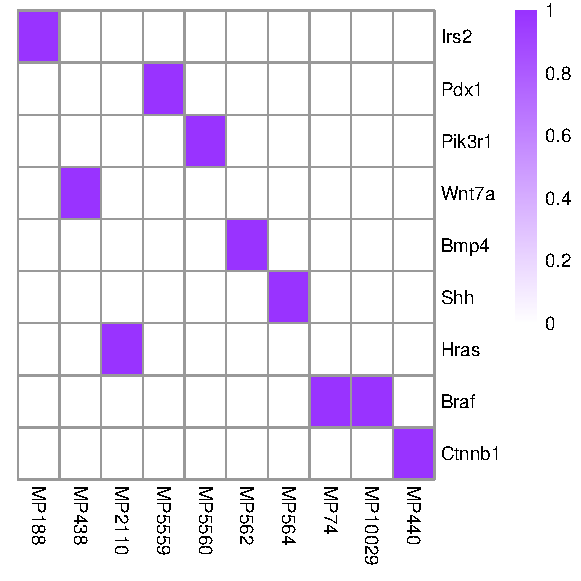
\includegraphics[width=\linewidth]{DrawPictures/v_4.pdf}
    \centerline{(a)}
  \end{minipage}
   \begin{minipage}[b]{.45\linewidth}
   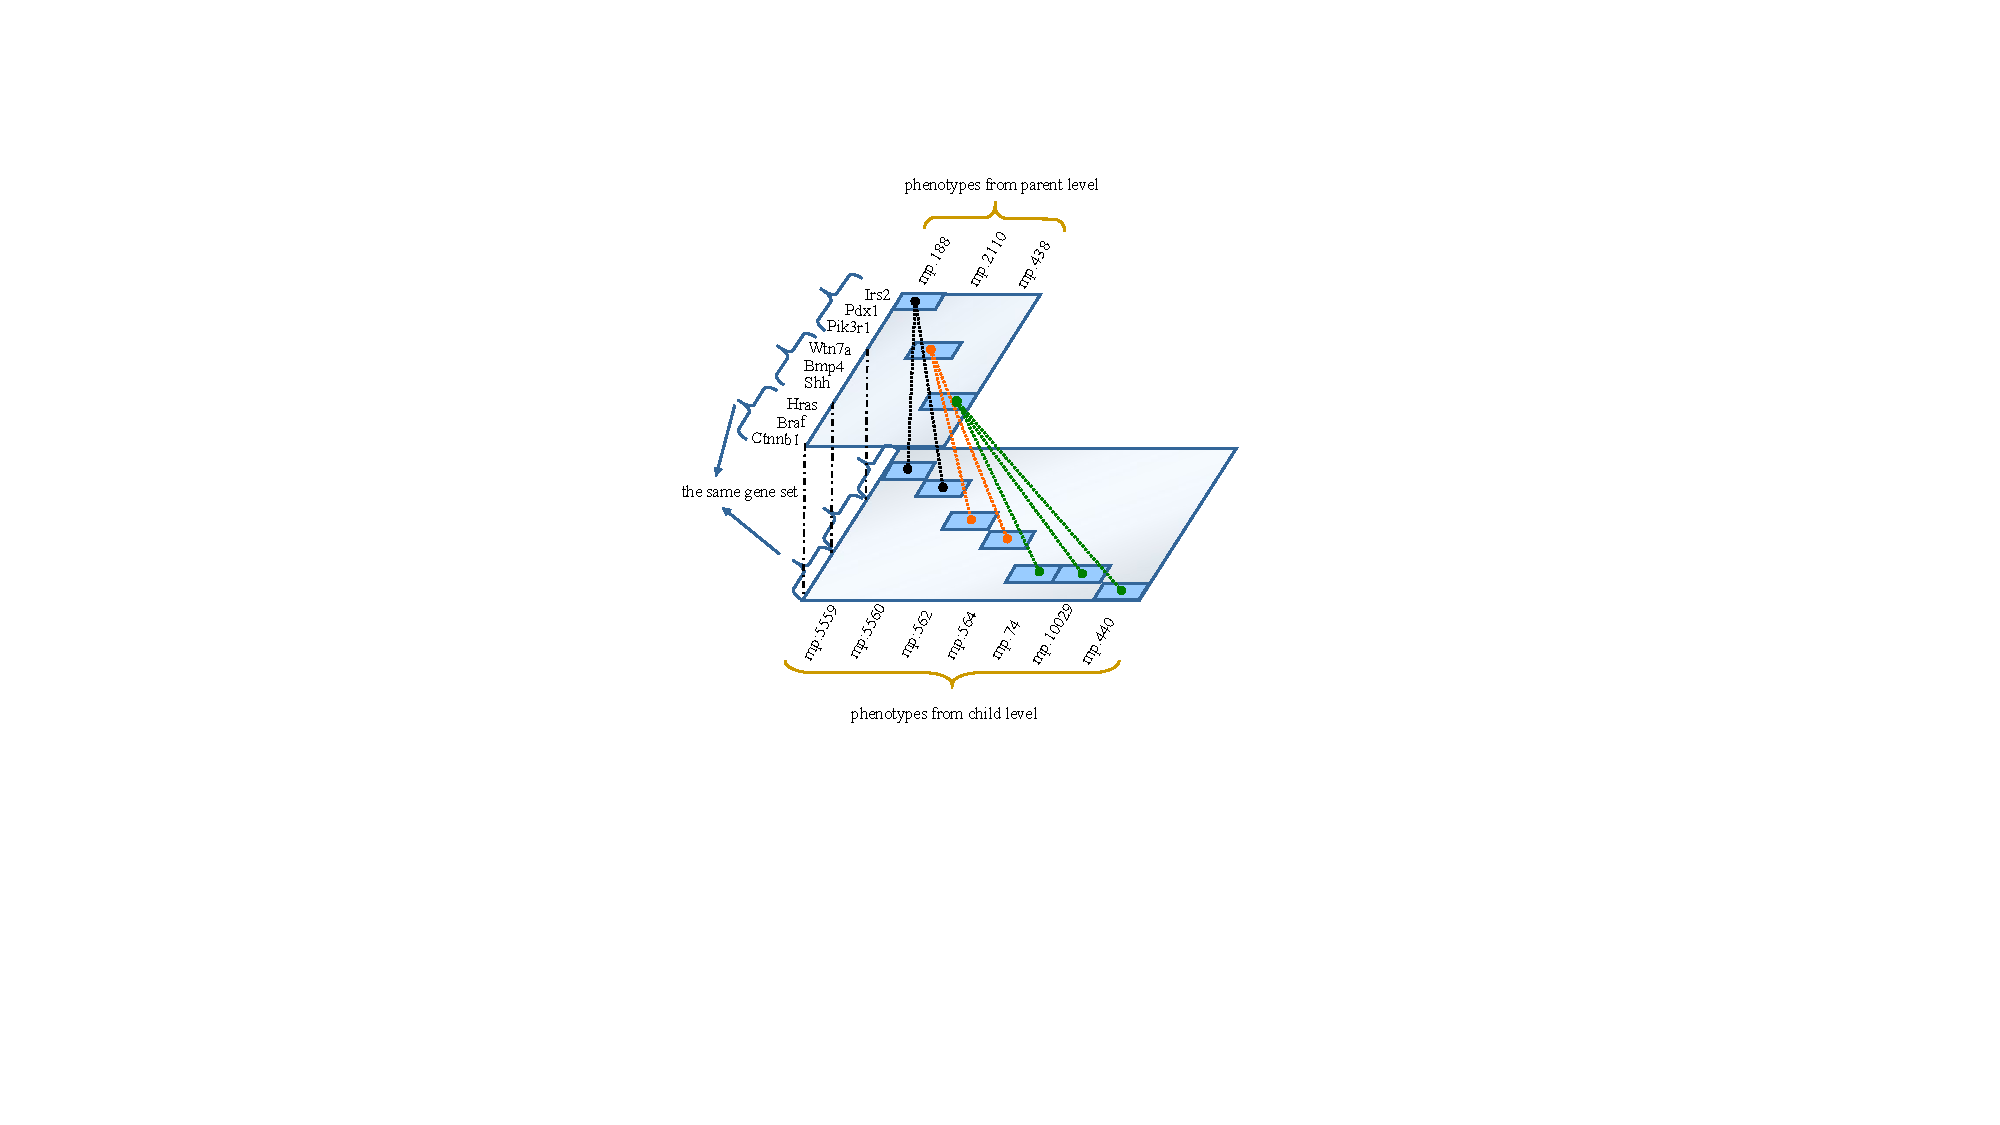
\includegraphics[width=\linewidth]{DrawPictures/Hierarchica.pdf}
    \centerline{(b)}
  \end{minipage}
  \vfil
  \begin{minipage}{.3\linewidth}
   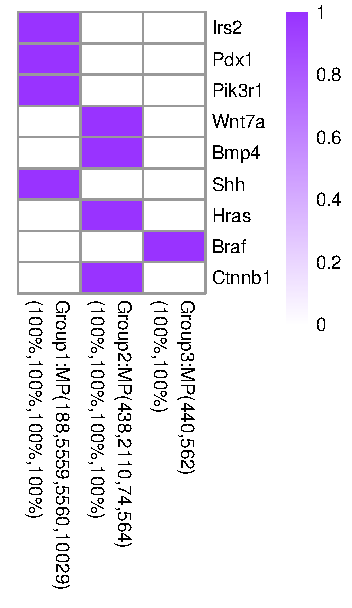
\includegraphics[width=\linewidth]{DrawPictures/v0.pdf}
    \centerline{(c)}
  \end{minipage}
  \hfil
  \begin{minipage}{.3\linewidth}
   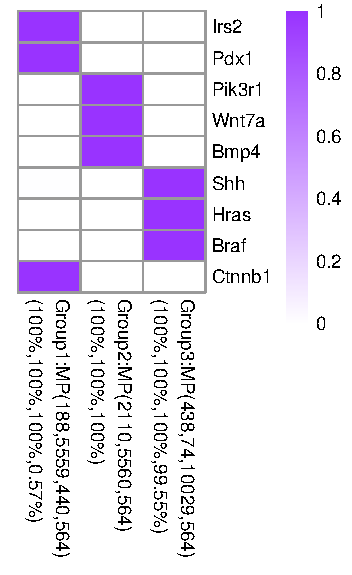
\includegraphics[width=\linewidth]{DrawPictures/v3.pdf}
    \centerline{(d)}
  \end{minipage}
  \hfil
  \begin{minipage}{.3\linewidth}
   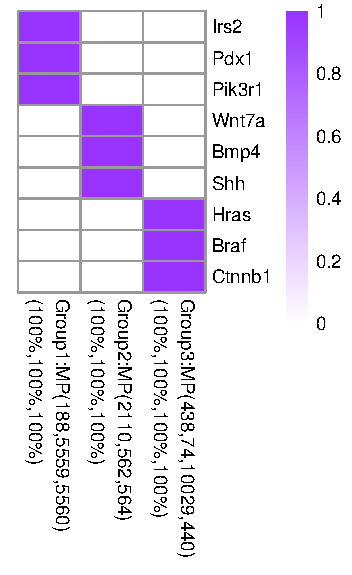
\includegraphics[width=\linewidth]{DrawPictures/v4.pdf}
    \centerline{(e)}
  \end{minipage}
  \caption{Illustration of sampled data, rows stand for genes, columns stand for \protect\\
  phenotype. If there is a association between a gene and a phenotype, the \protect \\
  corresponding position is colored, otherwise it's uncolored. (a) a overview of \protect \\
  association matrix of sampled data; (b) Illustration of hierarchical information \protect \\
  of phenotype ontology we used in our model; (c) Clustering result of HMF; (d)\protect \\
  Clustering result of CMNMF($\gamma$=1). In (c) and (d), each group is characterized \protect \\
  with phenotypes, which are classified to groups after the convergence. We also \protect \\
  show how much percent of each phenotype takes within a group.}
  \label{fig:sampled_result}
\end{figure}
 We sampled gene-phenotype association matrix and hierarchical mapping relations from real data to illustrate the usage of the hierarchical information. Figure \ref{fig:sampled_result}(a) is a overview of the sampled data matrix; Figure \ref{fig:sampled_result}(b) illustrates the hierarchical information we used in CMNMF, the upper matrix means the associations between genes and phenotypes from parent level, the lower matrix means the associations between genes and phenotypes from child level, the different color dash lines means parent-child phenotype relationships in different groups.
%The three phenotypes used in $A_1$ are from parent level, the other six phenotypes used in $A_2$ are from child level. Fig.\ref{fig:sampled_raw_data}(c) is a overview of all genes and phenotypes, we denote this data as $(A_3)_{9\times9}$.
To be more specific, we sampled the common nine genes from three groups (Irs2, Pdx1, Pik3r1 are from pathway mmu7930, \emph{i.e.} type-\uppercase\expandafter{\romannumeral2} diabetes mellitus; Hras, Braf, Ctnnb1 are from pathway mmu5212, \emph{i.e.} prostate cancer; Wnt7a, Bmp4, Shh are from pathway mmu5217, \emph{i.e.} Basal cell carcinoma). For each group, there are two genes associating with phenotypes in the child level (like in Figure \ref{fig:sampled_result}(b), Pdx1 and Pik3r1, from pathway mmu7930, are interacting with MP5559, MP5560, which are in the child level of the phenotype ontology hierarchical tree), and another gene associating with the parent phenotypes (Irs2, from pathway mmu7930, is interacting with MP188, which is in the parent level). The task is to cluster the three genes, which are coming from the same pathway, into a same group.

%%%%%%%%%%%%%%%%%%%%%%%%%
  We apply HMF and our model CMNMF to the sampled data, conducting each experiment 20 times and show average result in Figure \ref{fig:sampled_result}(c) and (d) respectively. Figure \ref{fig:sampled_result}(c) tells the fact that we use a common basis matrix $G$ while factorizing $A_1$ and $A_2$ simultaneously, we can see that in each gene group module, there exists misclassified genes(such like, Ctnnb1 shouldn't be grouped with Irs2 and Pdx1, it's supposed to classified with Hras and Braf). After we adding the hierarchical information to our model, just as Figure \ref{fig:sampled_result}(d) shows, all the genes are classified into three groups perfectly. It demonstrates that the two constraints working together can get the best performance. The reasons for the performance improvement are that with the consistent constraint, CMNMF can incorporate information from two levels and take advantage of the complement characteristic of information from different levels to overcome the shortcoming of lacking enough information from only one level and the hierarchy mapping constraint can help restrict cluster results according to the structure of data which narrows the range of solution space so that we can get a better solution.

%\subsection*{\textbf{2 Functional gene module similarity analysis}}
%\begin{figure}[!h]
%  \centering
% \includegraphics[width=0.8\textwidth]{DrawPictures/pathwaySimi.eps}
%  \caption{$gene\ group\ in\ pathway's\ similarity\ under\ GO-term  $}\label{fig:alpha}
%\end{figure}

\subsection*{\textbf{Comparison with Baseline Methods by Mining Gene Modules}}
In this part, we evaluate the proposed CMNMF and baseline methods on MGI mouse gene-phenotype ontology association data.
CMNMF is executed to mine gene functional modules and it is compared with the following clustering methods: HAC (Hierarchical Agglomerative Clustering)\cite{Ward1963}, KMeans, Kernel-Kmeans\cite{Dhillon2004}, LDA\cite{Blei2003},NMF\cite{Mika1999} and HMF (Hierarchical Matrix Factorization) \cite{AliMashhoori2012}. To be fair, all matrix factorization-based methods are implemented with sparse and non-negative constraints. We measured the performance by the $F_1$ measure, $Jaccard\ Index$, $Rand\ index$, and $GO_{rate}$.

We combine the phenotypes from level 4 and level 5 as features for each genes, and apply this data to HAC, Kmeans, Kernel-Kmeans, LDA, and NMF. In HAC and Kmeans, we use the Euclidean distance as the gene similarity measure to cluster the genes; for Kernel-Kmeans, Gaussian Kernel function is used for calculating the gene similarity, there is a hyper-parameter $\sigma$ in Kernel-Kmeans, we search it in \{0.001,0.01,0.1,1,10\}; we set the values of hyper-parameters $\alpha$ and $\beta$ in LDA as \cite{Wei2006} suggested. Because there are common sparse constraints in NMF, HMF and CMNMF, we search the parameters $\lambda_1$, $\lambda_2$ in a grid \{0.001,0.01.0.1,0,1,10\}; in our proposed model CMNMF, there are two additional parameters $\alpha$ and $\gamma$, when $\gamma$ is set to zero, our model CMNMF degrades to HMF, we will give more discussions about how these two parameters affect the performance of CMNMF in the following parts.

For methods LDA, NMF, HMF, and CMNMF, the gene clustering results are row-normalized by using z-score. For each gene, it can belong to multiple clusters, as it can participate in a couple of pathways, so we take the following strategy to predict the clusters the gene belongs to. First, for a cluster distribution of a gene, we sort the values in a descending order; then we choose the top k clusters, of which the sum of the values is closest to 0.9, as the gene belongs to.

Follow the description above, we get the results of gene clustering. We use $n$ to denote the total gene number, all genes can be denoted as $S=\{O_1,...,O_n\}$, we use gene pathways $X=\{X_1,...,X_r\}$ as the ground-truth partition of genes, and use clustering result $Y=\{Y_1,...,Y_s\}$ as prediction partitions, then define the following notations: TP, TN, FN, FP, which are defined according to whether pairs of elements of $S$ are in $X$ and $Y$ or not
%\footnote{more details see: https://en.wikipedia.org/wiki/Rand\_index}.
%\begin{itemize}
%\item TP, the number of pairs of elements in $S$ that are in the same set in $X$ and in the same set in $Y$
%\item TN, the number of pairs of elements in $S$ that are in different sets in $X$ and in different sets in $Y$
%\item FN, the number of pairs of elements in $S$ that are in the same set in $X$ and in different sets in $Y$
%\item FP, the number of pairs of elements in $S$ that are in different sets in $X$ and in the same set in $Y$
%\end{itemize}
Now we can define the evaluation measures as below:
\begin{equation}\label{}\nonumber
\begin{split}
F_{1}\ measure&=\frac{2PR}{P+R}\quad(P=\frac{TP}{TP+FP},  R=\frac{TP}{TP+FN}) \\
Jaccard\ Index&=\frac{TP}{TP+FP+FN}\\
Rand\ Index&=\frac{TP+TN}{TP+FP+FN+TN}
\end{split}
\end{equation}
For all these three measurements $F_1\ measure$, $Jaccard\ Index$ and $Rand\ Index$, the higher values, the better clustering results.
%\begin{equation}
%\begin{split}
%IC(t_i)&=Specificity(t_i)\times{Coverage(t_i)}\\
%&=Specificity(t_i)\times{(1-\frac{\log(desc(t_i)+1)}{\log(total\_terms)})}
%\end{split}
%\end{equation}
%\begin{equation}
%\begin{split}
%FS_{simGIC}(G_A,G_B)=\frac{\sum_{t_i\in{T_A\bigcap{T_B}}}IC(t_i)}{\sum_{t_j\in{T_A\bigcup{T_B}}}IC(t_j)}
%\end{split}
%\end{equation}
Another measurement on gene ontology for prediction clustering result $Y=\{Y_1,...,Y_s\}$, we draw the similar concept from\cite{Wei2006}, using  $(Sim)_{between}$ to denote the average similarity between different gene clusters, $(Sim)_{between}$ to denote average similarity of different genes within gene clusters. then we defined $GO_{rate}$ as:
$$
GO_{rate} = \frac{(Sim)_{between}}{(Sim)_{within}}
$$
where
\begin{equation}\label{}\nonumber
\begin{split}
(Sim)_{between}&=\frac{1}{{|Y|\choose 2}}\sum_{\forall(i,j)\in P}
\frac{\sum_{k=1}^{|Y_i|}\sum_{l=1}^{|Y_j|}FS_{simGIC}(G_k,G_l)}{|Y_i||Y_j|}\\
(Sim)_{within}&=\frac{1}{|Y|}\sum_{i=1}^{|Y|}
\frac{\sum_{j=1}^{|Y_i|}\sum_{k=j+1}^{|Y_i|}FS_{simGIC}(G_j,G_k)}{{|Y_i|\choose 2}}
\end{split}
\end{equation}
,
$P=\{(i,j)|1\leq i< j\leq|Y|\}$, $FS_{simGIC}(G_k,G_l)$ \cite{Teng2013} is used to measure the similarity between gene $G_k$ and $G_l$ by GO terms. In terms of evaluation measure $GO_{rate}$ we defined here, the lower values, the better clustering results.
\begin{table}[!t]
\centering
\caption{Performance results of different methods on $F_1$, $Jaccard\ Index$, $Rand\ Index$, $GO_{rate}$}\label{tab:measurements}
\begin{tabular}{c|cccc}
\hline
&$F_1$ measure &Jaccard Index& Rand Index&$GO_{rate}$\\
\hline
HAC&0.0839&0.0438&0.9525&0.6608\\
%\hline
Kmeans&0.0536&0.0290&0.9683&0.7039\\
%\hline
Kernel-Kmeans&0.0594&0.0306&0.9677&0.7400\\
%\hline
LDA&0.0978&0.0525&0.9618&0.8614\\
%\hline
NMF&0.093&0.0488&\textbf{0.9740}&0.7664\\
%\hline
ColNMF&0.0942&0.0495&0.9738&0.7417\\
%\hline
CMNMF&\textbf{0.1065}& \textbf{0.0563}&{0.9701}& \textbf{0.6559}\\
\hline
\end{tabular}
\end{table}

The results of each evaluation measures are shown in Table \ref{tab:measurements}.
It's obvious from the table that our model CMNMF beats all the baselines in terms of $F_1$, $Jaccard\ Index$, and $GO_{rate}$, the results show that our model CMNMF, which considers the hierarchical information of phenotype ontology do have effect on clustering results. However on $Rand\ Index$, NMF outperforms other methods, we should be aware of that $Rand\ Index$ takes TN gene pairs into account, but the number of TN pairs is way great than others and dominates the result of $Rand\ Index$. As we all know, the point we care about is whether two genes co-occur in a pathway rather than two genes show up in different pathways, thus higher $Rand\ Index$ does not reflect the performance of clustering results.

\subsection*{\textbf{Parameter Tuning}}
\begin{figure}[!h]
  \begin{minipage}[t]{0.7\linewidth}
    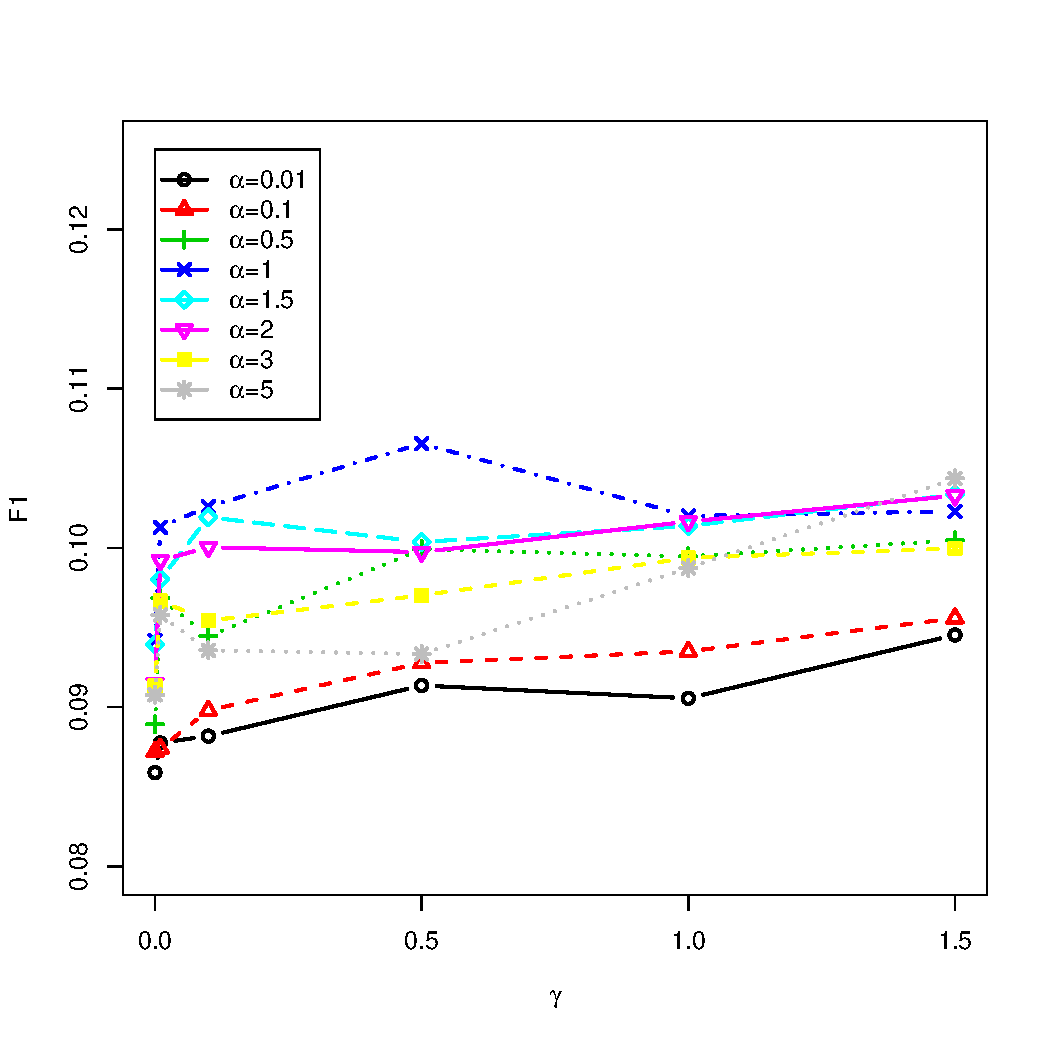
\includegraphics[width=\linewidth,origin = l]{DrawPictures/alpha-gamma.pdf}
  \end{minipage}
  \caption{$F_1$ score changes with $\gamma$ value in condition of different $\alpha$}
  \label{fig:alpha_gamma}
\end{figure}

In this part, we give discussions on how parameters $\alpha$ and $\gamma$ affect the clustering results. Because $F_1$ measure is a  harmonic average of precision and recall, it can avoid group lots of genes into a single cluster ,which is not the situation we are expecting.

The $\alpha$ in our CMNMF model, balances the contributions from different levels is an important parameter. When $\alpha$ is close to 0, the model degrades into NMF on level 4 and when $\alpha$ is big enough information from level 5 dominates the model. The $\gamma$ controls the effects of hierarchical information of phenotype ontologies, when $\gamma$ is set to 0, the models does not take hierarchical information into consideration, in this situation, our model degrades to HMF model, the higher $\gamma$ value, the more influence of hierarchical information has.
 The performance of CMNMF with different $\alpha$ and $\gamma$ is shown in Figure \ref{fig:alpha_gamma}. We search $\alpha$ in \{0.01 , 0.1 , 0.5, 1, 1.5, 2, 3, 5\} and $\gamma$ in \{0, 0.01,0.1,0.5,1,1.5\}, different color line stands the performance of $F_1$ under fixed $\alpha$ value and different $\gamma$ values.

It can be seen from Figure \ref{fig:alpha_gamma}, there is uprising trend with $\gamma$ growing under different $\alpha$ values, which demonstrates the hierarchical information has general positive effects. Especially, when $\gamma$ changes from 0 to 0.1, a steep improvement can be observed. After that, as $\gamma$ increasing, most lines have a gentle growth. In our model, the best performance of $F_1$ measure is achieved when $\alpha=1$ and $\gamma = 1.5$.

\subsection*{\textbf{Biological Analysis on Gene Modules}}%GO Enrichment

We used the DAVID\cite{Dennis2003} to investigate the enrichment of functional annotations of genes selected in each gene modules found by our model CMNMF. DAVID\footnote{https://david.ncifcrf.gov/summary.jsp} starts by reading the input file that contains a list of genes, and estimates the statistical significance of the enrichment of Gene-Ontology (GO) terms.
Table \ref{tab:GO_Enrichment} shows the enrichment of GO terms. We present some significant biological processes for certain  gene modules.


\begin{table}[!h]
\centering
\caption{Enrichment of GO categories in gene modules selected by CMNMF}\label{tab:GO_Enrichment}
\begin{tabular}{clll}
\hline
No &Genes in Module& Most Related GO Terms &P-value\\
\hline
\hline
\multirow{3}{*}{204}&
\multirow{3}{11em}{GCK, PDX1, INS2,\\E2F1, HNF1A,TNF, \\LEP, RPS6KA3,\\AKT2, SLC5A1, \emph{et al.}}&
 response to organic substance;&1.5E-08\\
 &&glucose metabolic process;&9.5E-07\\
 &&positive regulation of macromolecule-\\&& metabolic process;&1.6E-06\\
\hline
\multirow{3}{*}{201}&
\multirow{3}{11em}{AR, NFKBIA, CREBBP,\\CEBPA, DCC,VHL, \\SOS1, FLT3, FASL, \emph{et al.}}&
 hemopoietic or lymphoid organ development;&3.3E-17\\
 &&immune system development;&7.5E-17\\
 &&hemopoiesis;&1.5E-16\\
\hline
\multirow{3}{*}{138}&
\multirow{3}{11em}{GCK, SLC2A4, IRS1,\\INS2, IRS2, LDLR, LIPA,\\PCSK1, POMC, \emph{et al.}}&
 response to insulin stimulus;&2.8E-10\\
 &&response to hormone stimulus;&7.2E-10\\
 &&response to endogenous stimulus;&1.9E-09\\
\hline
\multirow{3}{*}{127}&
\multirow{3}{11em}{CDK4, ERCC1, G6PC,\\ GAD2,GHR, GPI1,\\ PDX1,MAFA, \emph{et al.}}&
 glucose metabolic process;&1.5E-07\\
 &&hexose metabolic process;&5.4E-07\\
 &&monosaccharide metabolic process;&1.2E-06\\
\hline
\multirow{3}{*}{41}&
\multirow{3}{11em}{FCGR2B, C1QA, C4B,\\TROVE2, LYN, POLB,\\WT1,LAMB2, \emph{et al.}}&
 immune effector process;&7.5E-06\\
 &&negative regulation of immune system process;&2.2E-05\\
 &&immune response;&5.9E-05\\
\hline
\multirow{3}{*}{13}&
\multirow{3}{11em}{MSH2,TSC2,PRKAR1A,\\VHl,CDKN2A,KRAS,\\FHIT,TRP53, \emph{et al.}}&
 regulation of cell proliferation;&2.9E-07\\
 &&negative regulation of cell proliferation;&4.3E-07\\
 &&regulation of apoptosis;&5.9E-06\\
\hline
\end{tabular}
\begin{tablenotes}
      \small
      \item The first column is the index of gene modules got by CMNMF, for each gene module, we present ten genes in the second column, and we put three most related GO terms and their corresponding P-values in the third and fourth column respectively.
    \end{tablenotes}
\end{table}

It's clear that in Table \ref{tab:GO_Enrichment}, gene modules found by CMNMF are statistical significant in terms of certain common GO terms (like: regulation of cell proliferation,immune response, et al.). Besides, we explore the relationships between genes in the modules and diseases in literature to demonstrate the biological meaning of modules found by CMNMF.

In gene module No.204, a number of genes are validated to be associated with diabetes. \cite{Haeusler2015} found that, in diabetic subjects with HbA1c $>$ 7.0, gluconeogenic enzymes were expressed normally, but GCK was suppressed more than 60\%. Moreover, HbA1c and fasting glucose were negatively correlated with GCK, but showed no correlation with G6PC, PCK1, or PCK2.
Through the studies of \cite{Herbach2007}, Munich INS2 (C95S) mutant mice are considered a valuable model to study the mechanisms of beta-cell dysfunction and death during the development of diabetes.
 In the study of \cite{Swaroop2012}, which revealed a significant correlation between TNF-$\alpha$ levels and BMI (P=0.006), the correlation being stronger in males when compared to females. A significant correlation was found between per cent $\beta$ cell function and TNF-$\alpha$ (P=0.008). TNF-$\alpha$ correlated significantly with HOMA IR, HOMA B and insulin, in type 2 diabetes.

In gene module No.201, we have found genes in this module have a strong relation to prostate cancer. To be more specific, Han \cite{Han2015} found that with the exception of NFKBIA 3' UTR polymorphism, the heterozygous and mutant genotypes of the other polymorphisms were significantly associated with prostate cancer risk, polymorphisms in NFKB1 and NFKBIA genes may modulate the risk of developing prostate cancer. \cite{Ding2014} developed functional evidence for CBP (Crebbp) and PTEN interaction in prostate cancer based on findings of their correlate expression in the human disease.  \cite{Timofeeva2009} established primary prostate cancer epithelial cells from 14 AA and 13 EA men, to identify cancer-specific gene expression patterns in AA men.
\cite{Tan2015} gave An overview of AR structure and activity, its actions in prostate cancer, and how structural information and high-throughput screening have been or can be used for drug discovery are provided herein.


 We can observe the similar phenomena in other gene modules\footnote{the overall gene modules got by CMNMF can be found in additional file xxx}, it could guide the researchers to study the relations between gene modules and some certain diseases. Our model CMNMF may inspire researchers to discover some underlying patterns behind the sophisticated biological system.
\subsection*{\textbf{Gene-Phenotype Association Prediction with Supervised CMNMF}}
When we add the gene pathways as a prior, the supervised CMNMF can also be used for gene-phenotype association prediction.In our experiments, we collected 229 mouse pathways from KEGG in total. We choose 21 common KEGG disease pathways (\emph{e.g.} alzheimer, diabetes, prostate cancer, \emph{et.al.}) on mouse, there are 145 member genes in these 21 KEGG disease pathways pathways.
\begin{figure}[!h]
  \begin{minipage}[t]{0.9\linewidth}
    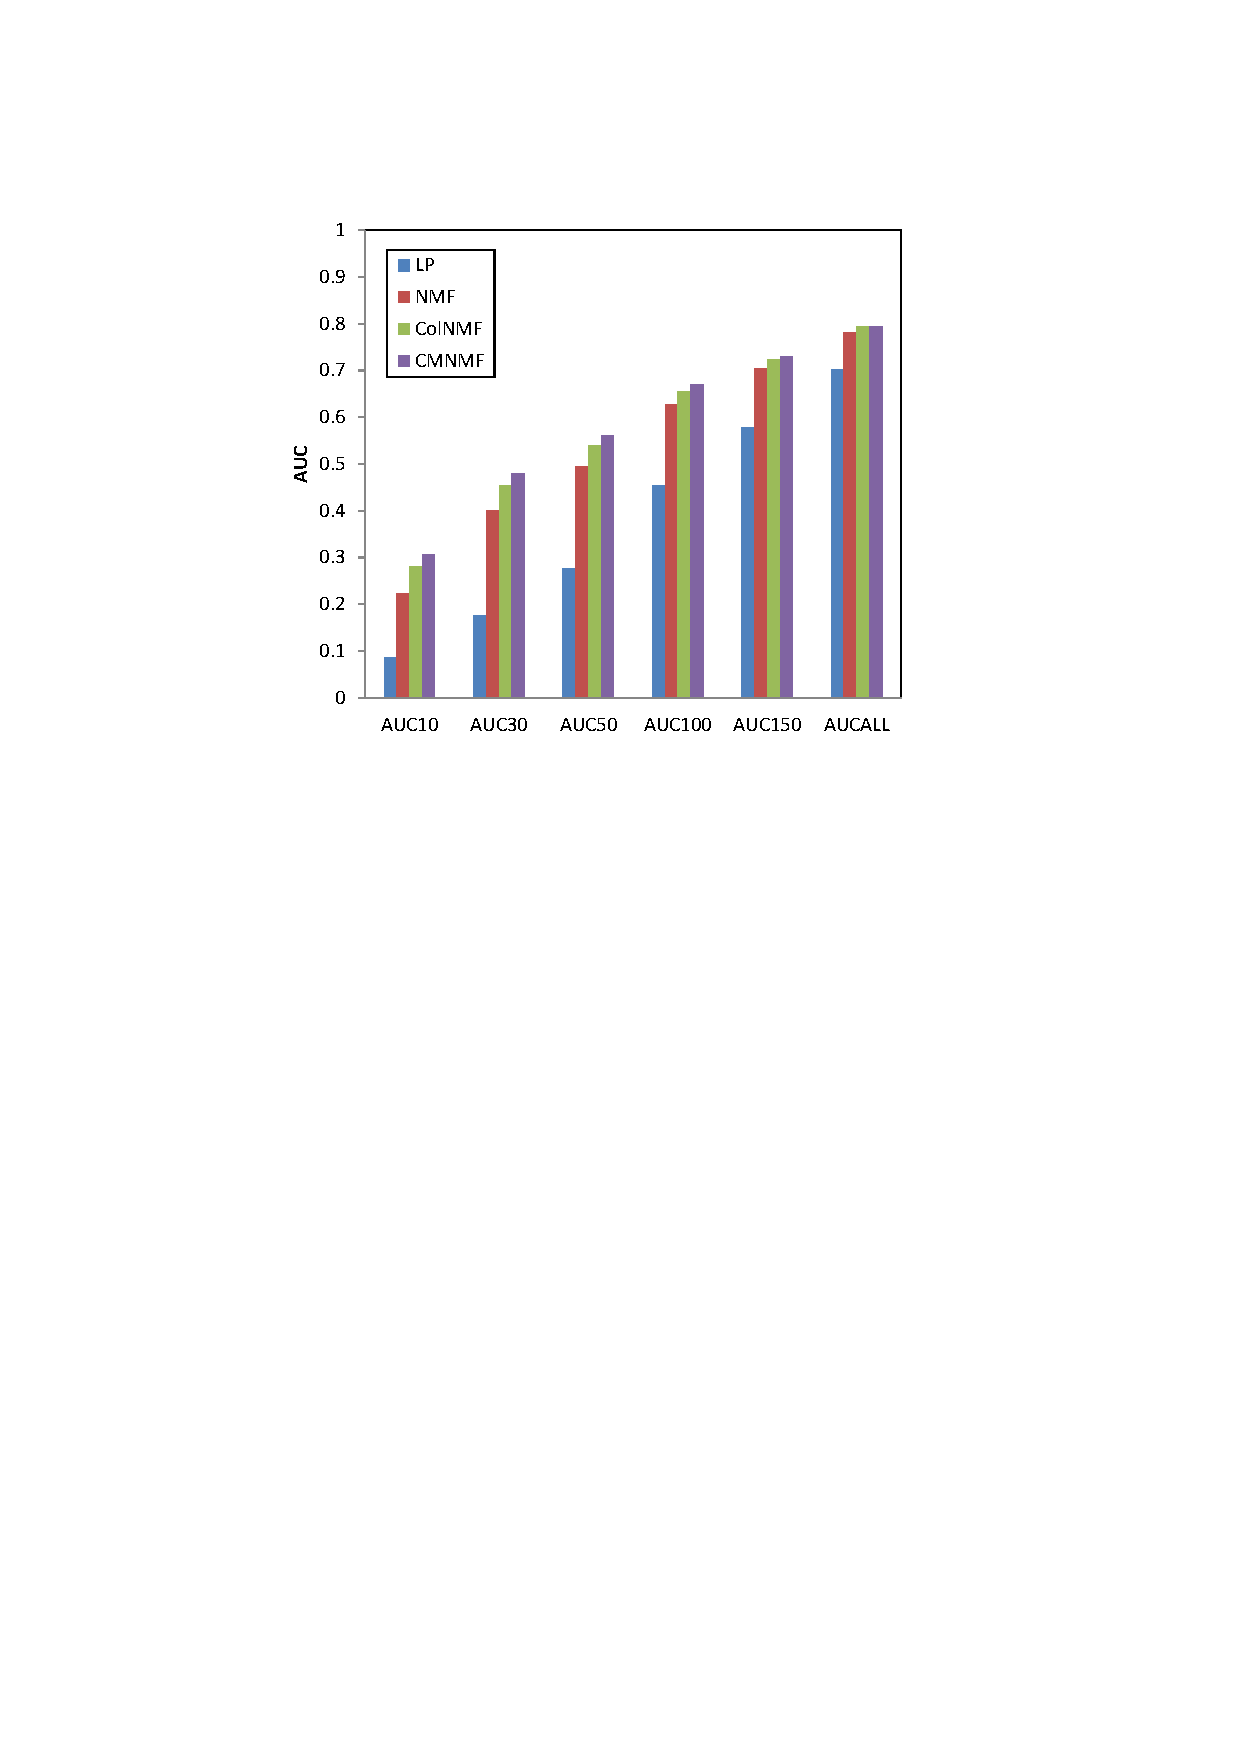
\includegraphics[width=\linewidth,origin = l]{DrawPictures/auc_excel.pdf}
  \end{minipage}
  \caption{AUC score of different method} \label{fig:AUC}
\end{figure}

 In the leave-one-out cross validation, each of the 145 member gene was held out and then classified into the 229 pathways as a multi-label classification problem since some of the disease genes are
members of multiple pathways. The higher the target pathways in the ranking of the 145 pathways, the better the performance. We measured the performance by the AUC. The baselines we use here is LP and HMF. LP was applied on the gene similarity network, in which the data be used was measured by genome-phenome association matrix. The other 144 member genes was used as the initialization of label propagations to classify the held-out gene. Another baseline is the HMF model we have introduced before. The average AUC score in the leave-one-out cross validation across the  member genes by all the methods are reported in Figure \ref{fig:AUC}. The results clearly show that our methods CMNMF takes advantage of LP and HMF, which only uses the genome-phenome association network for disease gene discovery.

\section*{Conclusions}
Gene modules play crucial roles in gene regulation, drug target identifying, and other aspects of application. As the advancements of technology and the expansions of data repositories, the quality and accessibility of data from a wide range of data sources will continuously increase. How to use these accumulated data in a proper way is still a challenging problem for researchers. It's important to design a framework to integrate different types of data for gene module discovery.

In this paper, we introduce a novel method, Consistent Multiple Nonnegative Matrix Factorization (CMNMF) based on genome-phenome association data factorization. Our approach was applied to an integration of hierarchical information of phenotype ontology, as far as we know, which has been rarely used in previous studies. The modules we found by our method express notable biological meaning.

There are several merits of our approach CMNMF. First, CMNMF keeps the gene cluster matrix consistent while it interacts with different phenotype ontology levels in decomposing data matrix; on the other hand, it restricts the similarity of phenotype pairs expressed in phenotype cluster matrix to satisfy the hierarchical structure. To achieve a better clustering results, we introduce sparse regularization on gene and phenotype decomposing matrix. The experiments result on our proposed method and other baselines (including HAC,Kmeans, kernel-Kmeans, LDA, NMF, HMF) show the effectiveness of our method. Furthermore, we give a more detailed discussion on the gene modules found by our method in biological aspects. Besides, we conduct a supervised CMNMF for gene-phenotype association prediction, the comparison of our model with LP and HMF demonstrate the good extension of our methods.

Although we have a trial on integration of hierarchical information of phenotype ontology on mouse for gene module discovery problem, there still exists a number of challenging issues to be solved. Such like: 1) In this work, we didn't give much talk on how to use the phenotype clustering results, because neither there has a clear definition of relationship between phenotypes, nor we have found a meaningful classification of phenotypes as a prior what we can utilize in our model; 2) at the moment, we are doing this research on mouse data, because there are much common characteristics between human and mouse, a key issue in the future is how to align the data between two species or even more in a framework to explore the understanding patterns of human biological mechanism; 3) as we know, gene clustering can also be conducted on a variety of gene expression data, here comes a fascinating question, is there possible to find an effective way to cluster genes by integrating genome-phenome data and expression data? Our work is just a snapshot of the biology system, we provide all our codes on Github website\footnote{\texttt{https://github.com/nkiip/CMNMF}\\} for interested researchers for future further investigations.

%%%%%%%%%%%%%%%%%%%%%%%%%%%%%%%%%%%%%%%%%%%%%%
%%                                          %%
%% Backmatter begins here                   %%
%%                                          %%
%%%%%%%%%%%%%%%%%%%%%%%%%%%%%%%%%%%%%%%%%%%%%%

\begin{backmatter}

\section*{Competing interests}
The authors declare that they have no competing interests.

\section*{Author's contributions}
MQX and YGZ originally design the model. YGZ worked on the method, experiment, analyses, and writing of the manuscript. YJX  contributed on method and analyses.  XF and YXH contributed on the experiment. ZCH contributed on the method. MQX and YLH contributed on writing of the manuscript. All authors read and approved the final manuscript.\ldots

\section*{Acknowledgements}
This work is supported by the National Natural Science Foundation of China (No. 61300166 and No. 61105049), the Open Project Foundation of Information Technology Research Base of Civil Aviation Administration of China (CAAC-ITRB-201303 and CAAC-ITRB-201408), the Natural Science Foundation of Tianjin (No. 14JCQNJC00600), and the Science and Technology Planning Project of Tianjin (No. 13ZCZDGX01098).

%%%%%%%%%%%%%%%%%%%%%%%%%%%%%%%%%%%%%%%%%%%%%%%%%%%%%%%%%%%%%
%%                  The Bibliography                       %%
%%                                                         %%
%%  Bmc_mathpys.bst  will be used to                       %%
%%  create a .BBL file for submission.                     %%
%%  After submission of the .TEX file,                     %%
%%  you will be prompted to submit your .BBL file.         %%
%%                                                         %%
%%                                                         %%
%%  Note that the displayed Bibliography will not          %%
%%  necessarily be rendered by Latex exactly as specified  %%
%%  in the online Instructions for Authors.                %%
%%                                                         %%
%%%%%%%%%%%%%%%%%%%%%%%%%%%%%%%%%%%%%%%%%%%%%%%%%%%%%%%%%%%%%

% if your bibliography is in bibtex format, use those commands:
\bibliographystyle{bmc-mathphys} % Style BST file (bmc-mathphys, vancouver, spbasic).
\bibliography{bmc_CMNMF}      % Bibliography file (usually '*.bib' )
% for author-year bibliography (bmc-mathphys or spbasic)
% a) write to bib file (bmc-mathphys only)
% @settings{label, options="nameyear"}
% b) uncomment next line
%\nocite{label}

% or include bibliography directly:
% \begin{thebibliography}
% \bibitem{b1}
% \end{thebibliography}

%%%%%%%%%%%%%%%%%%%%%%%%%%%%%%%%%%%
%%                               %%
%% Figures                       %%
%%                               %%
%% NB: this is for captions and  %%
%% Titles. All graphics must be  %%
%% submitted separately and NOT  %%
%% included in the Tex document  %%
%%                               %%
%%%%%%%%%%%%%%%%%%%%%%%%%%%%%%%%%%%

%%
%% Do not use \listoffigures as most will included as separate files

%%%%%%%%%%%%%%%%%%%%%%%%%%%%%%%%%%%
%%                               %%
%% Tables                        %%
%%                               %%
%%%%%%%%%%%%%%%%%%%%%%%%%%%%%%%%%%%

%% Use of \listoftables is discouraged.
%%


%%%%%%%%%%%%%%%%%%%%%%%%%%%%%%%%%%%
%%                               %%
%% Additional Files              %%
%%                               %%
%%%%%%%%%%%%%%%%%%%%%%%%%%%%%%%%%%%

\section*{Additional Files}
  \subsection*{Additional file 1 --- Sample additional file title}
    Additional file descriptions text (including details of how to
    view the file, if it is in a non-standard format or the file extension).  This might
    refer to a multi-page table or a figure.

  \subsection*{Additional file 2 --- Sample additional file title}
    Additional file descriptions text.


\end{backmatter}
\end{document}
